\documentclass[12pt,a4paper]{article}
\usepackage[T1]{fontenc}
\usepackage[spanish]{babel}
\usepackage{geometry}
\geometry{margin=2.5cm}
\usepackage{amsmath, amssymb}
\usepackage{graphicx}
\usepackage{booktabs}
\usepackage{xcolor}
\usepackage{array}
\usepackage{fancyhdr}
\usepackage{hyperref}
\usepackage{xurl}
\usepackage{caption}
\usepackage[section]{placeins}
\usepackage[expansion=false]{microtype}
\graphicspath{{figures/}}

\hypersetup{
  colorlinks=true,
  linkcolor=blue!60!black,
  urlcolor=blue!60!black,
  pdftitle={Evaluacion Practica Unidad 2 - Monolito vs Microservicios},
  pdfauthor={Hernandez Barreto Alan Daleth; Alfonso Dominguez Gonzales},
}

\pagestyle{fancy}
\fancyhf{}
\setlength{\headheight}{15pt}
\lhead{Examen Unidad 2 -- Fundamentos de Ciencia de Datos}
\rhead{}
\cfoot{\thepage}

\newcommand{\fuentep}{\par\vspace{2pt}\footnotesize\textit{Fuente: elaboración propia.}\par}

\title{\textbf{Evaluación Práctica de la Unidad 2}\\[4pt]
\large Inferencia Estadística y Toma de Decisiones en Ingeniería\\[2pt]
\normalsize Caso A: Arquitectura de Software (Monolito vs. Microservicios)}
\author{Hernandez Barreto Alan Daleth \\ Alfonso Dominguez Gonzales\\[6pt]
TecNM -- Departamento de Sistemas y Computación\\
Ingeniería en Sistemas Computacionales\\
Asignatura: Fundamentos de Ciencia de Datos}
\date{Octubre 2026}

\begin{document}
\maketitle
\thispagestyle{empty}

\begin{abstract}
Se evalúa si la sobrecarga de red de una arquitectura de microservicios incrementa la latencia de respuesta HTTP respecto a un monolito. A partir de un dataset sintético de 500 observaciones (250 por grupo) depurado con el criterio $1{,}5\times$IQR (483 registros), se aplicaron estadística descriptiva, simulación del Teorema Central del Límite (TCL), intervalos de confianza y una prueba t de Student bilateral. El IC al 95\% para la diferencia de medias fue $[-9{,}63,\ 6{,}80]$ ms y la prueba arrojó $t=-0{,}34$ con $p=0{,}74$: no se rechaza la hipótesis nula. La latencia media no difiere significativamente entre arquitecturas en este experimento.
\end{abstract}

\section{Introducción y objetivo}
En sistemas distribuidos se presume que la comunicación entre servicios agrega latencia frente a un despliegue monolítico. El objetivo de este trabajo es someter esa premisa a un contraste estadístico formal, usando Python (numpy \cite{harris2020numpy}, pandas \cite{mckinney2010pandas}, matplotlib \cite{hunter2007matplotlib}, seaborn \cite{waskom2021seaborn}, scipy \cite{virtanen2020scipy}) sobre la variable \emph{latencia de respuesta HTTP (ms)} agrupada por \emph{tipo de arquitectura} (Monolito vs. Microservicios), y emitir una recomendación técnica de ingeniería respaldada por un nivel de significancia $\alpha = 0{,}05$.

\section{Metodología}
\subsection{Dataset}
Conjunto sintético paramétrico justificado ($N = 500$, semilla 42). Las latencias se modelan con distribuciones gamma de cola derecha, típicas de tiempos de servicio de red, más un piso mínimo de procesamiento local:
\begin{align*}
Y_{\text{monolito}} &= \Gamma(k=2{,}5,\ \theta=35) + 40, &\qquad Y_{\text{micro}} &= \Gamma(k=2{,}2,\ \theta=40) + 45,\\
\mathbb{E}[Y_{\text{monolito}}] &= 127{,}5\ \text{ms}, &\qquad \mathbb{E}[Y_{\text{micro}}] &= 133\ \text{ms}.
\end{align*}
El grupo microservicios usa menor forma ($k$: 2,5 $\rightarrow$ 2,2) y mayor escala ($\theta$: 35 $\rightarrow$ 40) para representar mayor varianza por saltos de red y serialización. Los datos crudos y depurados se alojan en \texttt{data/} y el cuaderno ejecutable en \texttt{notebooks/}.

\subsection{Tratamiento de atípicos}
Para cada grupo se calcula el rango intercuartílico $\mathrm{IQR}=Q_3-Q_1$; se eliminan observaciones fuera de $[Q_1-1{,}5\,\mathrm{IQR},\ Q_3+1{,}5\,\mathrm{IQR}]$. Resultado: 17 atípicos (10 Monolito, 7 Microservicios), $N_{\text{dep}}=483$.

\subsection{Métodos estadísticos}
Los criterios de inferencia siguen la práctica estándar de ingeniería \cite{montgomery2021applied, wasserman2004all}:
\begin{itemize}
\item Error estándar de la media: $\sigma_{\bar x} = s/\sqrt{n}$; verificación empírica con $k=1000$ remuestreos con reemplazo para $n\in\{5,15,30,60\}$.
\item Intervalo de confianza para $\mu$: $\bar x \pm t_{\alpha/2,\,n-1}\cdot s/\sqrt{n}$. Se usa t-Student porque $\sigma$ es desconocida y se sustituye por $s$; para $n\geq30$ es asintóticamente equivalente a Z.
\item Diferencia de medias: si Levene no rechaza homogeneidad ($p\geq0{,}05$), varianzas combinadas $s_p^2=\frac{(n_1-1)s_1^2+(n_2-1)s_2^2}{n_1+n_2-2}$; en caso contrario, corrección de Welch con grados de libertad de Satterthwaite.
\item Contraste bilateral de medias mediante \texttt{scipy.stats.ttest\_ind}, con hipótesis $H_0:\ \mu_1=\mu_2$ frente a $H_1:\ \mu_1\neq\mu_2$.
\end{itemize}

\section{Bloque 1: Estadística descriptiva y limpieza}
Tras la depuración, los estadísticos por grupo son:
\begin{table}[htbp]
\centering
\caption{Estadísticos descriptivos de la latencia (ms) por arquitectura ($N_{\text{dep}}=483$).}
\begin{tabular}{lrrrrrr}
\toprule
Grupo & $\bar x$ & Mediana & $s$ & $s^2$ & Asimetría & Curtosis \\
\midrule
Monolito & 123,200 & 117,012 & 43,529 & 1894,787 & 0,616 & $-0,159$ \\
Microservicios & 124,614 & 113,969 & 48,204 & 2323,634 & 0,770 & $-0,094$ \\
\bottomrule
\end{tabular}
\fuentep
\end{table}

Ambas distribuciones presentan asimetría positiva (cola derecha), coherente con colas de latencia de red, y curtosis cercana a cero (colas menos pesadas que la normal). Microservicios muestra mayor dispersión ($s=48{,}20$ vs.\ $43{,}53$ ms). En los histogramas con KDE (Figura~\ref{fig:hist}) se aprecia el solapamiento sustancial de ambas poblaciones; los boxplots (Figura~\ref{fig:box}) confirman medianas y rangos comparables.

\begin{figure}[htbp]
\centering
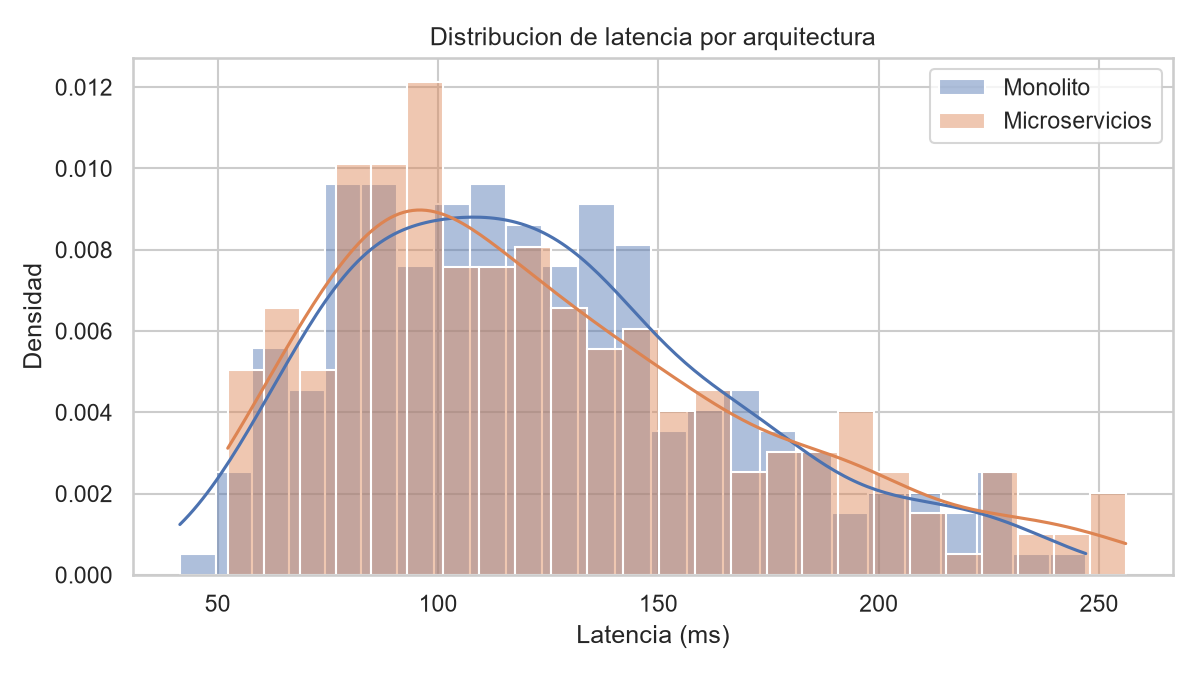
\includegraphics[width=0.85\textwidth]{histogramas_kde.png}
\caption{Histogramas con densidad KDE de la latencia por arquitectura.}
\label{fig:hist}
\fuentep
\end{figure}

\begin{figure}[htbp]
\centering
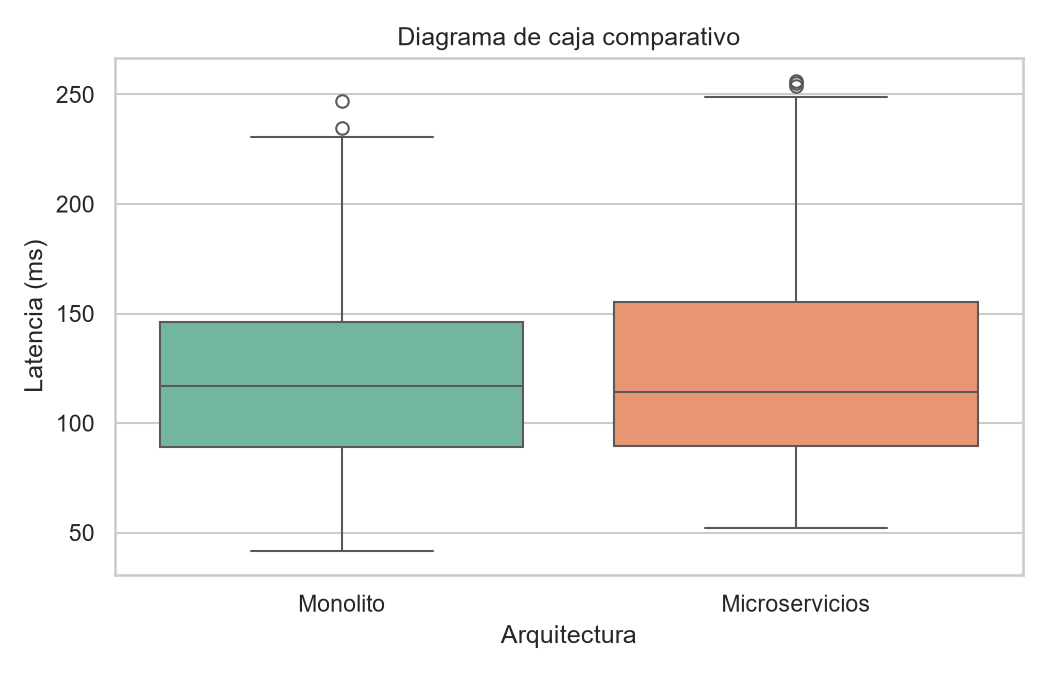
\includegraphics[width=0.7\textwidth]{boxplots.png}
\caption{Diagramas de caja comparativos por arquitectura.}
\label{fig:box}
\fuentep
\end{figure}

\section{Bloque 2: Teorema Central del Límite}
Se extrajeron $k=1000$ medias muestrales con reemplazo para cada $n\in\{5,15,30,60\}$ a partir de la muestra global depurada ($\bar x = 123{,}91$ ms, $s = 45{,}90$ ms). La cuadrícula de la Figura~\ref{fig:tcl} muestra cómo las medias se concentran y ganan simetría al aumentar $n$.

\begin{figure}[htbp]
\centering
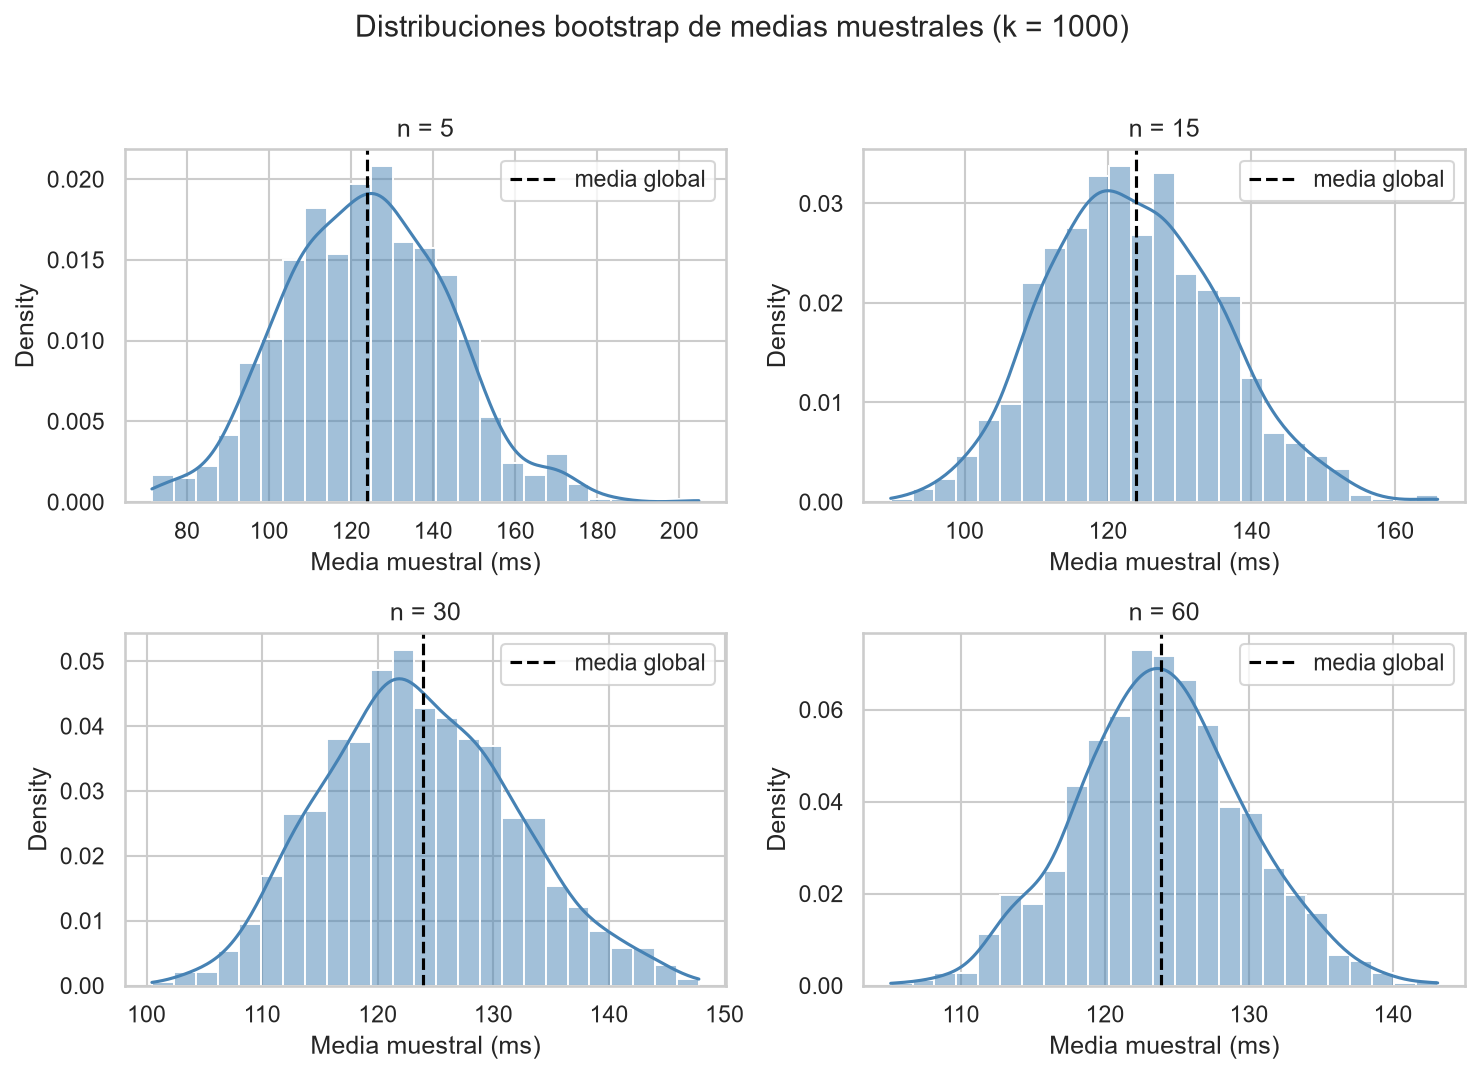
\includegraphics[width=0.9\textwidth]{tcl_grid.png}
\caption{Distribuciones bootstrap de medias muestrales ($k=1000$).}
\label{fig:tcl}
\fuentep
\end{figure}

\begin{table}[htbp]
\centering
\caption{Error estándar empírico vs.\ teórico $s/\sqrt{n}$.}
\begin{tabular}{rrrrr}
\toprule
$n$ & Media de medias & SE empírico & SE teórico & Diferencia (\%) \\
\midrule
5 & 123,918 & 19,886 & 20,526 & 3,12 \\
15 & 123,615 & 11,932 & 11,851 & 0,68 \\
30 & 123,658 & 8,236 & 8,380 & 1,72 \\
60 & 123,882 & 5,860 & 5,926 & 1,11 \\
\bottomrule
\end{tabular}
\fuentep
\end{table}

El SE empírico difiere del teórico en menos de 3,2\% en todos los casos, validando la forma $\sigma_{\bar x}=s/\sqrt{n}$. Las distribuciones muestrales de medias convergen a la normal conforme crece $n$, evidencia directa del TCL aun partiendo de poblaciones asimétricas.

\section{Bloque 3: Intervalos de confianza}
\subsection{Media general}
Usando t-Student con $n=483$ ($\sigma$ desconocida):
\begin{table}[htbp]
\centering
\caption{Intervalos de confianza para la media general de latencia (ms).}
\begin{tabular}{lrr}
\toprule
Confianza & Límite inferior & Límite superior \\
\midrule
90\% & 120,470 & 127,353 \\
95\% & 119,808 & 128,015 \\
99\% & 118,511 & 129,312 \\
\bottomrule
\end{tabular}
\fuentep
\end{table}

\subsection{Diferencia de medias}
La prueba de Levene obtuvo $W=1{,}8419$ con $p=0{,}1754\geq0{,}05$: no se rechaza la homogeneidad de varianzas, por lo que se usa el estimador de varianzas combinadas con $n_1+n_2-2=481$ grados de libertad:
\[
(\bar x_1-\bar x_2)\ \pm\ t_{0{,}025,\,481}\cdot s_p\sqrt{\tfrac{1}{n_1}+\tfrac{1}{n_2}}
\ =\ -1{,}414 \ \pm\ 8{,}21 \ =\ [-9{,}63,\ 6{,}80]\ \text{ms}.
\]
El valor cero pertenece al intervalo ($0\in IC$): a nivel poblacional la diferencia $\mu_{\text{Monolito}}-\mu_{\text{Microservicios}}$ perfectamente puede ser nula. Prácticamente no existe evidencia de que la arquitectura de microservicios agregue latencia media en este experimento; cualquier diferencia observable es compatible con el ruido muestral.

\section{Bloque 4: Teoría de decisión}
\subsection{Planteamiento}
\[
H_0:\ \mu_{\text{Monolito}}=\mu_{\text{Microservicios}}
\qquad\text{vs.}\qquad
H_1:\ \mu_{\text{Monolito}}\neq\mu_{\text{Microservicios}},
\quad \alpha=0{,}05.
\]

\subsection{Matriz de decisión y costos}
\begin{table}[htbp]
\centering
\caption{Matriz de decisión con costo operativo de cada error.}
\small
\begin{tabular}{>{\raggedright\arraybackslash}p{3.2cm}>{\raggedright\arraybackslash}p{2.6cm}>{\raggedright\arraybackslash}p{2.4cm}>{\raggedright\arraybackslash}p{5.2cm}}
\toprule
$H$ verdadera & Decisión & Resultado & Costo / consecuencia técnica \\
\midrule
$H_0$ & Rechazar $H_0$ & Error Tipo I ($\alpha$) & Migrar a microservicios sin beneficio medible: mayor complejidad operativa e infraestructura. \\
$H_0$ & No rechazar $H_0$ & Correcta ($1-\alpha$) & Se conserva el monolito con evidencia de ausencia de sobrecarga significativa. \\
$H_1$ & Rechazar $H_0$ & Correcta ($1-\beta$) & Migración justificada: se absorbe la sobrecarga planificando latencia. \\
$H_1$ & No rechazar $H_0$ & Error Tipo II ($\beta$) & No migrar existiendo sobrecarga real: latencia evitable en producción. \\
\bottomrule
\end{tabular}
\fuentep
\end{table}

\subsection{Resultado y veredicto}
Con \texttt{scipy.stats.ttest\_ind} (varianzas combinadas, $n_1=240$, $n_2=243$):
\[
t = -0{,}3384, \qquad p\text{-valor} = 0{,}7352.
\]
Como $p = 0{,}7352 \geq \alpha = 0{,}05$, el veredicto es \textbf{no rechazar $H_0$}. No hay evidencia estadística de diferencia en la latencia media entre monolito y microservicios; el IC de la diferencia lo confirma al contener al cero.

\subsection{Recomendación técnica}
La decisión de arquitectura debe sustentarse en criterios de escalabilidad, despliegue independiente y resiliencia, no en la latencia media observada. Si se migra a microservicios, se recomienda instrumentar telemetría de latencia en producción y dimensionar una tolerancia de hasta $\sim$10 ms de sobrecarga potencial, margen sugerido por el valor absoluto del límite inferior del IC 95\% de la diferencia ($|-9{,}63|\approx10$ ms); el límite superior ($+6{,}80$ ms) indica que microservicios incluso podría ser marginalmente más rápido.

\section{Reproducibilidad}
Todo el análisis es reproducible de extremo a extremo:
\begin{itemize}
\item Entorno verificado: Python 3.14.7, numpy 2.5.4, pandas 3.0.6, scipy 1.18.1, matplotlib 3.11.2, seaborn 0.13.2; resultados idénticos en el kernel de Kaggle (Python 3.13) y en Python 3.10 con numpy 2.2.
\item Semilla fija: \texttt{np.random.seed(42)} en la primera celda del cuaderno.
\item Ejecución local (raíz del repositorio): \texttt{jupyter nbconvert --to notebook --execute} sobre \path{notebooks/examen_fcd_u2.ipynb}.
\item Ejecución en la nube: \url{https://www.kaggle.com/code/dlthhb/examen-fcd-u2-monolito-vs-microservicios}.
\item Entregables en el repositorio: \texttt{data/} (CSV original y depurado), \texttt{notebooks/} (cuaderno con salidas), \texttt{docs/} (este reporte y figuras).
\end{itemize}

\section{Limitaciones}
\begin{itemize}
\item Con $n_1=240$, $n_2=243$ y $s_p\approx45{,}9$ ms, el tamaño muestral detecta con 80\% de potencia diferencias de magnitud $\gtrsim11{,}7$ ms; diferencias menores quedarían no detectadas.
\item No rechazar $H_0$ no demuestra equivalencia: solo indica ausencia de evidencia de diferencia. Para afirmar equivalencia se requeriría un diseño de hipótesis de equivalencia (TOST) con un margen práctico definido.
\item Los datos son sintéticos: los parámetros capturan el comportamiento esperado de latencias de red, pero la validez externa frente a cargas reales de producción no está garantizada.
\end{itemize}

\section{Conclusiones}
\begin{enumerate}
\item La limpieza con $1{,}5\times$IQR eliminó 17 atípicos (3,4\%); los estadísticos descriptivos revelan asimetría positiva moderada en ambos grupos.
\item La simulación del TCL ($k=1000$) verificó que el SE empírico coincide con $s/\sqrt{n}$ (diferencias $<3{,}2\%$) y que las medias muestrales convergen a la normal.
\item El IC 95\% para $\mu_{\text{Monolito}}-\mu_{\text{Microservicios}}$ es $[-9{,}63,\ 6{,}80]$ ms: contiene al cero.
\item Con $\alpha=0{,}05$, la prueba t ($p=0{,}74$) no rechaza $H_0$. Técnicamente, la sobrecarga de red de microservicios no demuestra un incremento significativo de latencia en este escenario.
\end{enumerate}

\bibliographystyle{plain}
\bibliography{referencias}

\end{document}
